% !TeX root = ../main.tex
% Add the above to each chapter to make compiling the PDF easier in some editors.
\chapter{Methodology}\label{chapter:method}
\section{Overall Aggregation Approach}
In order to avoid having a central raw data set and to eliminate the risk of inference attacks on anonymized data, we propose a framework which collects and locally aggregates location data on end-user devices (smartphones) through an application designed for this purpose. The raw data will stay on each device and will only be used to serve aggregation requests initiated by a central server. The aggregation requests have to be defined upfront. Apart from GPS data, we also take other movement data into account - the number of steps and the current activity e.g. walking. These can be used to enrich the pure GPS data. Hence, an example of an aggregation is the determination of the average number of steps per day across all users participating in the respective aggregation. An exemplary aggregation request sent to a smartphone is depicted in Fig. \ref{incoming-aggregation-request}. It specifies the timespan which should be covered by the aggregation, the type of aggregation and the current data combined in the ongoing aggregation.

\begin{figure}[h!]
	\begin{lstlisting}[language=json,firstnumber=1]
	{
		"start": "2019-05-30",
		"end": "2019-06-02",
		"type": "steps",
		"n" : 3,
		"value": 2000
	}
	\end{lstlisting}
	\caption{Exemplary body of an aggregation request to be served.}
	\label{incoming-aggregation-request}
\end{figure}

\begin{figure}[h!]
	\begin{lstlisting}[language=json,firstnumber=1]
	{
		"n" : 4,
		"value": 2500
	}
	\end{lstlisting}
	\caption{Exemplary response to an aggregation request.}
	\label{outgoing-aggregation-response}
\end{figure}

The response sent back to the server after processing the request only needs to contain the data itself, as the type and timespan can be inferred by the server from the request identifier. Figure \ref{outgoing-aggregation-response} shows an exemplary response to the server that matches the request in Fig. \ref{incoming-aggregation-request}.


\begin{figure}[h!]
	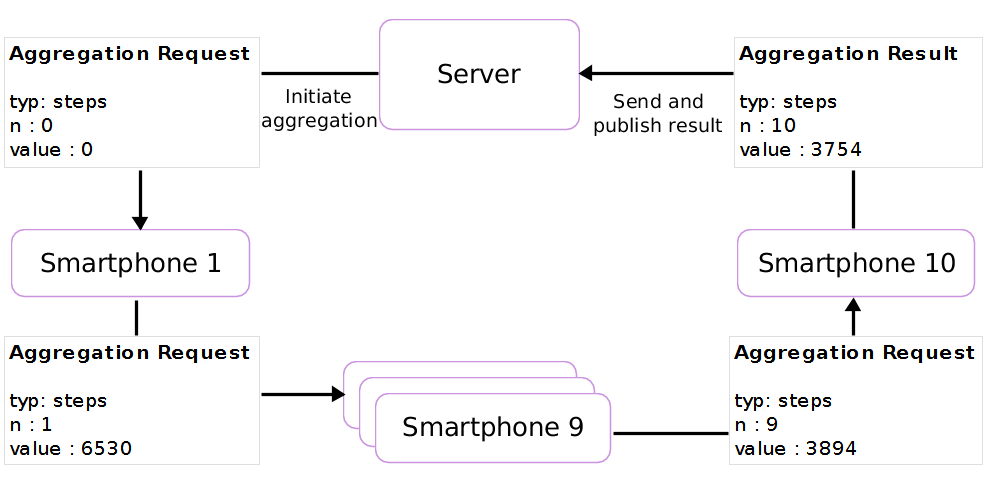
\includegraphics[width=\textwidth]{data/diagrams/decentral-aggregation-6.png}
	\caption{Overview of the decentral unencrypted aggregation process via P2P.}
	\label{decentral-aggregation-unencrypted}
\end{figure}

Figure \ref{decentral-aggregation-unencrypted} depicts the overall process of such a decentral aggregation request using an example of 10 participating devices.
In order to protect the user's privacy and completely shield the raw data from the server, it would be necessary to pass the request via P2P from one device to another until the last device finally sends the results to the server. On the one hand, P2P on mobile phones, especially when sending larger messages, is still hardly possible. Similar to our approach, Eittenberger et al. \parencite{eittenberger2012rapidstream} use a central server to maintain the P2P network and Nurminen et al. propose the use of SMS obtain the IP address of the P2P partner \parencite{nurminen2006p2p}. Only when devices are locally close to each other, a P2P connection can be established directly using WIFI or Bluetooth \parencite{p2p-android}. On the other hand, if the server is used to pass an aggregation request from one device to another, it could read the data and compute the respective user's input from the difference. We propose to use encryption in order to hinder the server from reading the data and assume the server to be trusted in the first place. Chapter \ref{chapter:conclusion} discusses this limitation. The modified aggregation process using encryption is depicted in Fig. \ref{decentral-aggregation-encrypted}. On installation of the application on a smartphone, a public-private key-pair is generated and every installed application registers at the server with this public key. In order to provide more anonymity, this public-private key-pair could also be exchanged regularly similar to the approach of mix-nodes by [CITE!!!]. The corresponding private key is stored only locally. On the start of an aggregation request, not only the first user but also the subsequent user in the chain of users who should deal with the aggregation request is determined and the public key of this user is passed along with the aggregation request. When one end user device needs to send the processed aggregation request to the next phone, it encrypts the data using the provided public key of the next user leveraging the benefits of synchronous keys using the standard hybrid encryption approach\footnote{In hybrid encryption as used e.g. in SSL, the message itself is encrypted with a synchronous key while this key itself is encrypted using the public key.}. This way, the next phone in the aggregation chain will be able to decrypt the request and process the data while the server is unable to read the data until the aggregation request is finally sent in plain text for publishing to the server. 

 \begin{figure}[h!]
	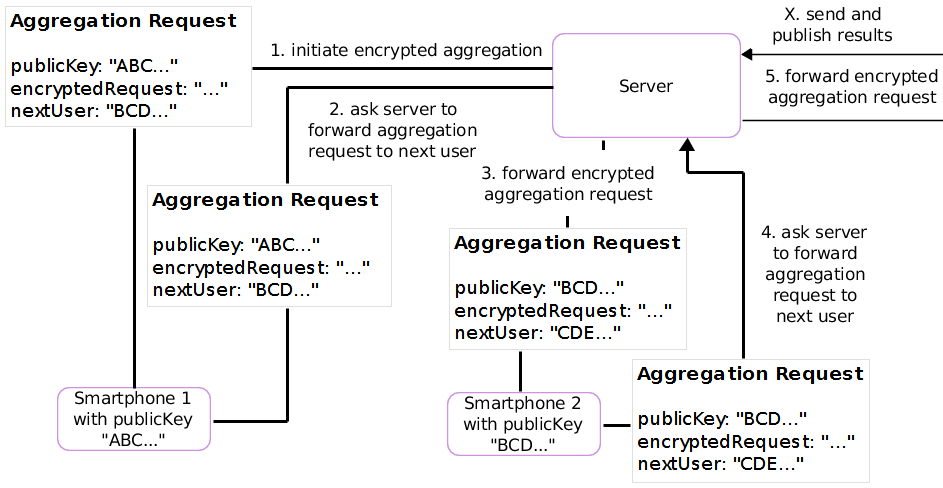
\includegraphics[width=\textwidth]{data/diagrams/decentral-encrypted-aggregation.png}
	\caption{Excerpt of the decentral encrypted aggregation process using a central server for message passing.}
	\label{decentral-aggregation-encrypted}
\end{figure}

 The aggregated results are planned to be available through a public route on the server. Nevertheless, we restrict access in our test run to our research team in order to protect the research participants' privacy in case there is a privacy risk we have not thought of. The aggregation requests themselves are initiated by our research team but can be initiated automatically on a regular basis in the future. The next section will detail the planned aggregations.

 \section{Aggregation Schemes}\label{aggregation-schemes}per
 Two types of aggregation requests are of special interest in our research. First, the aggregation of mean values and second, the aggregation of more advanced statistical values such as median or distribution function. The latter includes the possibility to calculate the former but requires the simultaneous availability of every single user's response. 
 The following list is an excerpt of aggregations that would be of interest and can be computed based on GPS location data in combination with the number of steps and the current activity of the respective person:
 \begin{enumerate}
 	\item The average number of steps walked across all users participating in the request. (e.g. to calculate how many people reach e.g. 10.000 steps per day\footnote{It has to be evaluated, which percentage of steps are usually registered because the phone will not always be carried the person.}.)
	\item The average time spent walking, running, in a vehicle or on a bicycle.
	\item The share of people who combine using a bicycle and using a vehicle within one trip.
	\item The time spent at work and the time it takes people to travel to work.
	\item Locations where many participants spend a significant amount of time on a certain day. (i.e. a posteriori event recognition.)
	\item The percentage of their overall travelling time that people spend on their bike, car, etc.
	\item The average speed on roads.
	\item The share of people who go to work by car, bike, etc. or a mixture of these.
 \end{enumerate}
 For all aggregations, always both, the mean value and if possible, a complete list of single users' mean values in order to compute other statistical figures, are of interest.

 \section{Limiting the Spatial Area of an Aggregation Request}
 The aggregation requests outlined in the former subsection only provide useful data if the area of the aggregation can be limited e.g. to the scope of a city. Otherwise, the resulting data would not allow for comparison. Furthermore, the scope of each aggregation would either be the whole user base or the limited number of participants in each aggregation would not necessarily be locally close to each other. The former might result in a huge amount of data being passed around, especially in the case of listing values, the latter would often make aggregations impossible because some aggregations like the average speed on roads require a certain number of participants providing data about the respective area. 
 In order to limit the area of an aggregation and avoid sending the aggregation request to every single user, leaving him with determining whether he can provide data about the respective, the initiator of those requests has to know the area, for which a user can provide data.
 We do not see this as a violation of the user's privacy due to the following reason: The exact location of the user e.g. the home or work location is not of interest at all. Rather the area for which the user can provide data is of interest. We propose to cluster location areas in a hierarchical structure similar to Mokbel et al. \parencite{casper} and determine the granularity of the location published to the server as follows:
\begin{enumerate}
	\item Each user sends the most coarse locational area possible to the server - e.g. the continent.
	\item If more than the required anonymity threshold of e.g. 10 active users are already registered with this area at the server, the server not only links this location to the user but also requests the user to send a less coarse location.
	\item The user step by step sends a less coarse location e.g country, district, etc. until the server denies to link the user to the area because not enough active users have registered with the location on this granularity level. The server nevertheless increases the counter of users who requested access to this area. Once the counter exceeds a certain number, the server sends an aggregation request to all participants in the more coarse area that encompasses the requested less coarse area to verify the number of active users. If this number is above the required threshold, the granularity level for this location is made available and users can now register with this area and aggregation requests targeting this area can be sent.
	\item The fulfilment of the threshold has to be checked on a regular basis in order to close areas once the user base sinks below the anonymity threshold.
\end{enumerate}
In a more advanced setting, it should be possible to register with more than one area on the same level to avoid that a user e.g. living close to a city provides data only about the city or the bordering area but not both. Nevertheless, this should be limited to areas bordering each other to avoid user identification similar as in Golle et al. \parencite{privacy-home-work-pairs}. Also, it has to be investigated whether this indeed does not pose a privacy risk to the user or whether also the combination of areas and not only each of the combined areas needs to meet a certain anonymity threshold.